\documentclass[12pt,a4paper,UTF8]{article}
\usepackage{ctex} % Chinese support
\usepackage{graphicx} % Insert images
\usepackage{subfigure}
\usepackage{float}
\usepackage{listings} % Print source code
\usepackage{color} % Color support
\usepackage{booktabs} % Professional table support
\usepackage{pdflscape} % Landscape pages support in PDF
\usepackage{hyperref} % Hypertext links support for cross-referencing
\usepackage{amsmath,mathtools}
\usepackage{ulem} % strikethrough

% Customize hyperref format (it's set to no special format here)
\hypersetup{hidelinks}

% Declare directories to search for graphics files for graphicx
\graphicspath{{figures/}}

% Define source code style for listings
\lstdefinestyle{verilog-style}{
	language=Verilog,
	basicstyle=\ttfamily\footnotesize,
	keywordstyle=\bfseries\color[rgb]{0, 0, 1},
	identifierstyle=\color[rgb]{0.5, 0.3, 0.1},
	stringstyle=\color[rgb]{0.6, 0.1, 0.1},
	commentstyle=\itshape\color[rgb]{0.05, 0.5, 0.05},
	backgroundcolor=\color[gray]{0.95},
	numbers=left,
	numbersep=5pt,
	numberstyle=\color[gray]{0.6},
  breaklines=true,
  escapeinside=``
}

\newcommand{\reporttitle}[2]{
  \LARGE\textsf{#1}\quad\underline{\makebox[12em]{#2}}
}

\newcommand{\reportinfo}[2]{
  \large\makebox[4em]{\textsf{#1}}\quad\underline{\makebox[18em]{#2}}
}

\begin{document}
\begin{titlepage}
  \centering
  \vspace*{\fill}
  {\Huge\textsf{数字电路与数字系统实验}} \\ [100pt]
  \reportinfo{实验名称}{exp05 计数器和时钟} \\ [10pt]
  \reportinfo{院系}{计算机科学与技术系} \\ [10pt]
  \reportinfo{学生姓名}{} \\ [10pt]
  \reportinfo{学号}{} \\ [10pt]
  \reportinfo{班级}{数字电路与数字系统实验1班} \\ [10pt]
  \reportinfo{邮箱}{} \\ [10pt]
  \reportinfo{实验时间}{2020 年 9 月 25 日} \\ [10pt]
  \vspace*{\fill}
\end{titlepage}
\tableofcontents
\newpage

\section{实验目的}
\begin{itemize}
  \item 学会用Verilog设计计数器和时钟
  \item 学习使用FPGA开发板上的时钟信号
\end{itemize}

\section{实验原理}
\begin{itemize}
  \item 利用触发器可以构成简单的计数器,即在
        每个CLOCK的上升沿计数器输出值加一
  \item 定时器的原理:
        \begin{equation}
          \mbox{计时时间} = \mbox{脉冲个数}\times \mbox{脉冲周期}
        \end{equation}
        \hspace*{2em}分频器可以用定时器的原理来解释:我们用的是
        FPGA开发板上50MHZ的时钟信号,脉冲周期为
        $\frac{1}{50M}$秒。对于我们要设置的以1秒为周期的
        时钟信号而言,计时时间为1秒,所以我们每秒需要
        50M个系统脉冲。也就是说,对于我们要设置的时钟信号,
        每经过25M个系统脉冲需要对它取一次反,使它每0.5秒产生一个
        上升沿或下降沿。
        \hspace*{2em}计时器的原理也是如此。例如实验5.4.1,我们
        要设计一个从00计数到99的计数器,计时时间为100。我们设置的
        时钟信号周期为1秒,所以需要经过100个时钟脉冲,
        然后计时结束,重新从零计数。
\end{itemize}

\section{实验环境/器材}
\begin{itemize}
  \item Quartus编辑器和DE10-Standard开发平台
  \item FPGA开发板
\end{itemize}

\section{程序代码+实验过程+测试方法}
\subsection{实验5.4.1 00$\sim$99计时器}
\subsubsection{实验代码}
我们要实现一个从00计数到99的计时器,要求此计时器有开始、暂停
和清零功能,并且计时结束时让一个发光二极管闪烁。那么,对于FPGA
开发板,我们需要系统的时钟信号;需要Switch开关来模拟开始、暂停
和清零按钮;需要LEDR发光二极管来产生计时结束的闪烁;需要
七段数码管来显示00$\sim$99的计数。

因为开始和暂停可以用一个开关来模拟,所以我让SW[0]模拟这个功能,
然后传入子模块用参数pause表示。SW[1]是清零开关,传入到参数clr。
LEDR[1]是计时结束的信号,对应参数RCO。我另外用LEDR[0]表示暂停信号,
在计数暂停时发亮,对应参数sign\_pause。系统的时钟信号传入到参数
clk\_sys。两个七段数码管分别对应参数Y\_tens和Y\_ones。
\begin{lstlisting}[style=verilog-style]
module counter_100(clk_sys, clr, pause, sign_pause, RCO, Y_tens, Y_ones);
	input clk_sys, clr, pause;
	output reg sign_pause, RCO;
	output reg [6:0] Y_tens, Y_ones;
\end{lstlisting}

另外我们还需要自定义的以1秒为周期的时钟信号clk\_1s,以及计数
系统脉冲是否达到25M的寄存器count\_clk。生成1秒时钟的代码
见实验5.3.2题目。这里回答一下实验5.3.2提出的问题:为了满足计数到
25M的要求,因为$2^{24}<25M<2^{25}$,所以count\_clk的宽度至少25位。
\begin{lstlisting}[style=verilog-style]
reg clk_1s;
reg [24:0] count_clk; 
integer count;
\end{lstlisting}

此外,我们还需要一个整数变量count,用来储存计数结果。这样就能在
always块中用case语句根据count选择七段数码管输出。根据实验5.2的提示,
我们需要在initial块中对各个变量和输出结果初始化,以免在仿真运行时出现
未定义的值。为了让实验报告有详有略,initial块和生成1秒时钟的always块
(见实验5.3.2题目)的代码就省略不贴出了。

然后,在每个1秒时钟的上升沿,我们对count操作并输出到七段数码管上:
\begin{lstlisting}[style=verilog-style]
always @ (posedge clk_1s) begin
  if (clr)                        count <= 0;
  else if (~pause && count == 99) count <= 0;
  else if (~pause)                count <= count + 1;
  else                            count <= count;

  case (count / 10)
    0 : Y_tens <= 7'b1000000;
    1 : Y_tens <= 7'b1111001;
    2 : Y_tens <= 7'b0100100;
    3 : Y_tens <= 7'b0110000;
    4 : Y_tens <= 7'b0011001;
    5 : Y_tens <= 7'b0010010;
    6 : Y_tens <= 7'b0000010;
    7 : Y_tens <= 7'b1111000;
    8 : Y_tens <= 7'b0000000;
    9 : Y_tens <= 7'b0010000;
    default: Y_tens <= 7'bx;
  endcase
  case (count % 10)
    0 : Y_ones <= 7'b1000000;
    1 : Y_ones <= 7'b1111001;
    2 : Y_ones <= 7'b0100100;
    3 : Y_ones <= 7'b0110000;
    4 : Y_ones <= 7'b0011001;
    5 : Y_ones <= 7'b0010010;
    6 : Y_ones <= 7'b0000010;
    7 : Y_ones <= 7'b1111000;
    8 : Y_ones <= 7'b0000000;
    9 : Y_ones <= 7'b0010000;
    default: Y_ones <= 7'bx;
  endcase
end
\end{lstlisting}

最后是暂停信号和RCO信号:
\begin{lstlisting}[style=verilog-style]
always @ (count or pause)
  if (count == 99 && ~pause) RCO = 1;
  else                       RCO = 0;
  
always @ (pause)
  if (pause) sign_pause = 1;
  else       sign_pause = 0;
\end{lstlisting}

\subsubsection{测试文件}
测试代码比较简单,就是简单的测试一下清零和暂停,
然后跑一个周期(00$\sim$99),就不详细解释了。
唯一要解释的一点是,因为系统脉冲周期与我们要
设定的时钟周期数值差距有亿点点大(也不过就差了
2的24次方),所以如果按前文代码进行仿真的话,
我们需要经过千万个系统时钟周期才能仿真出1秒
(你以为对仿真图拖一分钟滚动条或者缩放千万倍
就能看到1秒以后的世界了吗?天真!0.01秒你都
看不到!因为这个软件根本不会仿真那么长时间,
不到5000个时钟周期它就停止仿真了)。

所以我们设置count\_clk计数到10就把自身清零,并且
把clk\_1s取反,然后测试代码和结果如下:
\begin{lstlisting}[style=verilog-style]
initial
begin
	CLOCK_50 = 0;
	SW[0] = 0; // pause
	SW[1] = 0; // clear
	#100;
	SW[1] = 1; // clear on
	#50;
	SW[1] = 0; // clear off
	#300;
	SW[0] = 1; // pause
	#100;
	SW[0] = 0; // continue
	#2000;

	$stop;
end 

always
begin
	#0.02 CLOCK_50 = 1; #0.5;
	CLOCK_50 = 0; #0.48;
end
\end{lstlisting}

\begin{figure}[H]
  \centering
  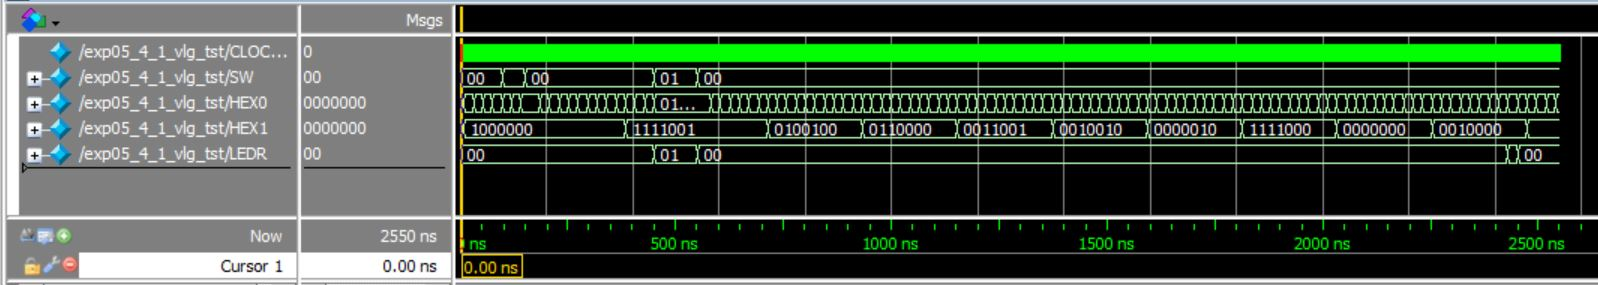
\includegraphics[width=1\textwidth]{1_sim.JPG}
  \caption{仿真运行}
  \label{1_sim}
\end{figure}

\subsection{实验5.4.2 电子时钟}
\subsubsection{实验代码}
在这个拓展实验中,我实现了以下功能:
\begin{enumerate}
  \item 一个显示时分秒的电子时钟
  \item 时钟的时间可调整
  \item 闹铃功能
\end{enumerate}

与实验5.4.1一样,我需要一些整数变量来储存时分秒,从而
用case语句选择输出到七段数码管。于是我创建了三个整数变量
count\_h, count\_min, count\_s。

对于调整时间的功能,我使用FPGA上的按钮来实现。4个按钮
KEY[3:0]\linebreak[4]传入到参数set\_acce[3:0],分别
对应调整使能、调整小时、调整分钟和调整秒数。
\begin{lstlisting}[style=verilog-style]
always @ (posedge clk_1s) begin
  if (~set_acce[3]) begin
    if (~set_acce[2]) count_h <= (count_h + 1) % 24;
    if (~set_acce[1]) count_min <= (count_min + 1) % 60;
    if (~set_acce[0]) count_s <= (count_s + 3) % 60;
  end

  else if (count_s == 59) begin
    count_s <= 0;
    if (count_min == 59) begin
      count_min <= 0;
      if (count_h == 23) count_h <= 0;
      else count_h <= count_h + 1;
    end else 
      count_min <= count_min + 1;
  end else
    count_s <= count_s + 1;

  /* `case语句省略` */
end
\end{lstlisting}

我用Switch开关模拟闹钟的设定,对应的传入参数是alarm\_clk。\linebreak[4]
alarm\_clk[9]控制闹钟使能,alarm\_clk[8:4]是闹钟的小时值,
alarm\_clk[3:0]是闹钟的分钟值。可设置的闹钟时间是5分钟的整数倍,
即alarm\_clk[3:0]对应的整数值的5倍就是所设闹钟的分钟值。闹钟的
持续时间为5分钟,闹钟期间LEDR[0]二极管会发光,以此表示闹钟时间到。
\begin{lstlisting}[style=verilog-style]
always @ (alarm_clk[9] or count_h or count_min or count_s)
	if (alarm_clk[9]) begin
		alarm_h = alarm_clk[8:4];
		alarm_min = alarm_clk[3:0];
		alarm_min = alarm_min * 5;
		if (alarm_h == count_h 
			&& count_min >= alarm_min 
			&& count_min < alarm_min + 5)
			sign_alarm = 1;
		else 
			sign_alarm = 0;
	end else
		sign_alarm = 0;
\end{lstlisting}

\subsubsection{测试文件}
先看仿真波形图,可以对测试文件的思路形成一个清晰的理解:
\begin{figure}[H]
  \centering
  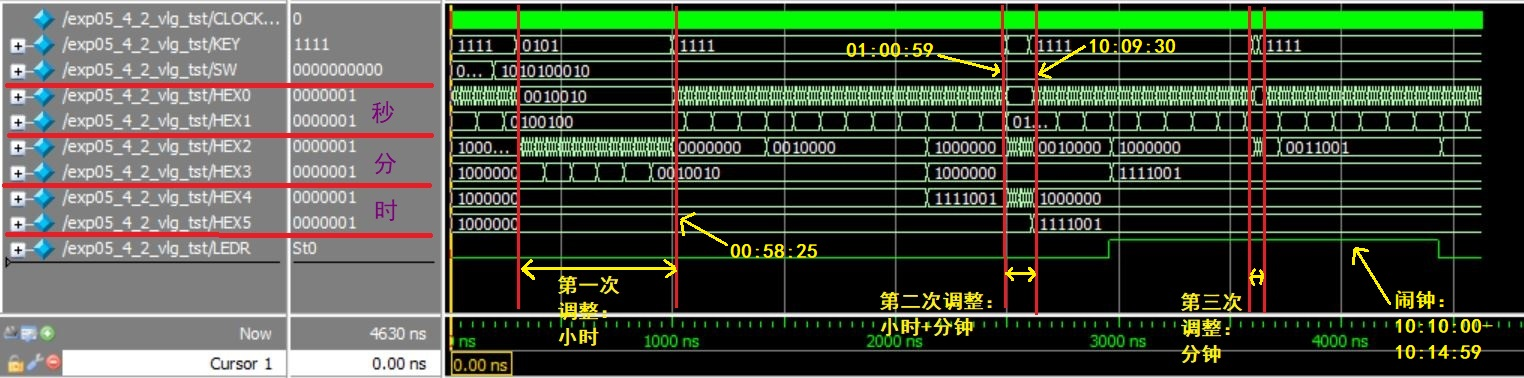
\includegraphics[width=1\textwidth]{2_sim.JPG}
  \caption{仿真运行}
  \label{2_sim}
\end{figure}

和实验5.4.1的测试文件一样,我们需要修改一下count\_clk。
这次我们计数到5就把count\_clk清零。然后测试代码如下:
\begin{lstlisting}[style=verilog-style]
initial
begin
	CLOCK_50 = 0;
	SW = 10'b0;
	KEY = 4'b1111;
	#200;
	SW = 10'b1010100010; // alarm at 10:10
	#100;
	KEY = 4'b0101; // set minute to 58 
	#700;
	KEY = 4'b1111; // normal clock
	#1500;         // it's 01:00:59 after 1500 clock cycles 
	KEY = 4'b0001; // set hour to 10; set minute to 09
	#100;
	KEY = 4'b1111; // normal clock, then the alarm 'rings'
	#1000;
	KEY = 4'b0101; // accelerate the minute hand
	#30;
	KEY = 4'b1111; // normal clock
	#1000;         // alarm clock ends
	$stop;
end

always
begin
	#0.02 CLOCK_50 = 1; #0.5;
	CLOCK_50 = 0; #0.48;
end
\end{lstlisting}

\section{实验结果}
在FPGA开发板上运行非常成功。
\begin{figure}[H]
  \centering
  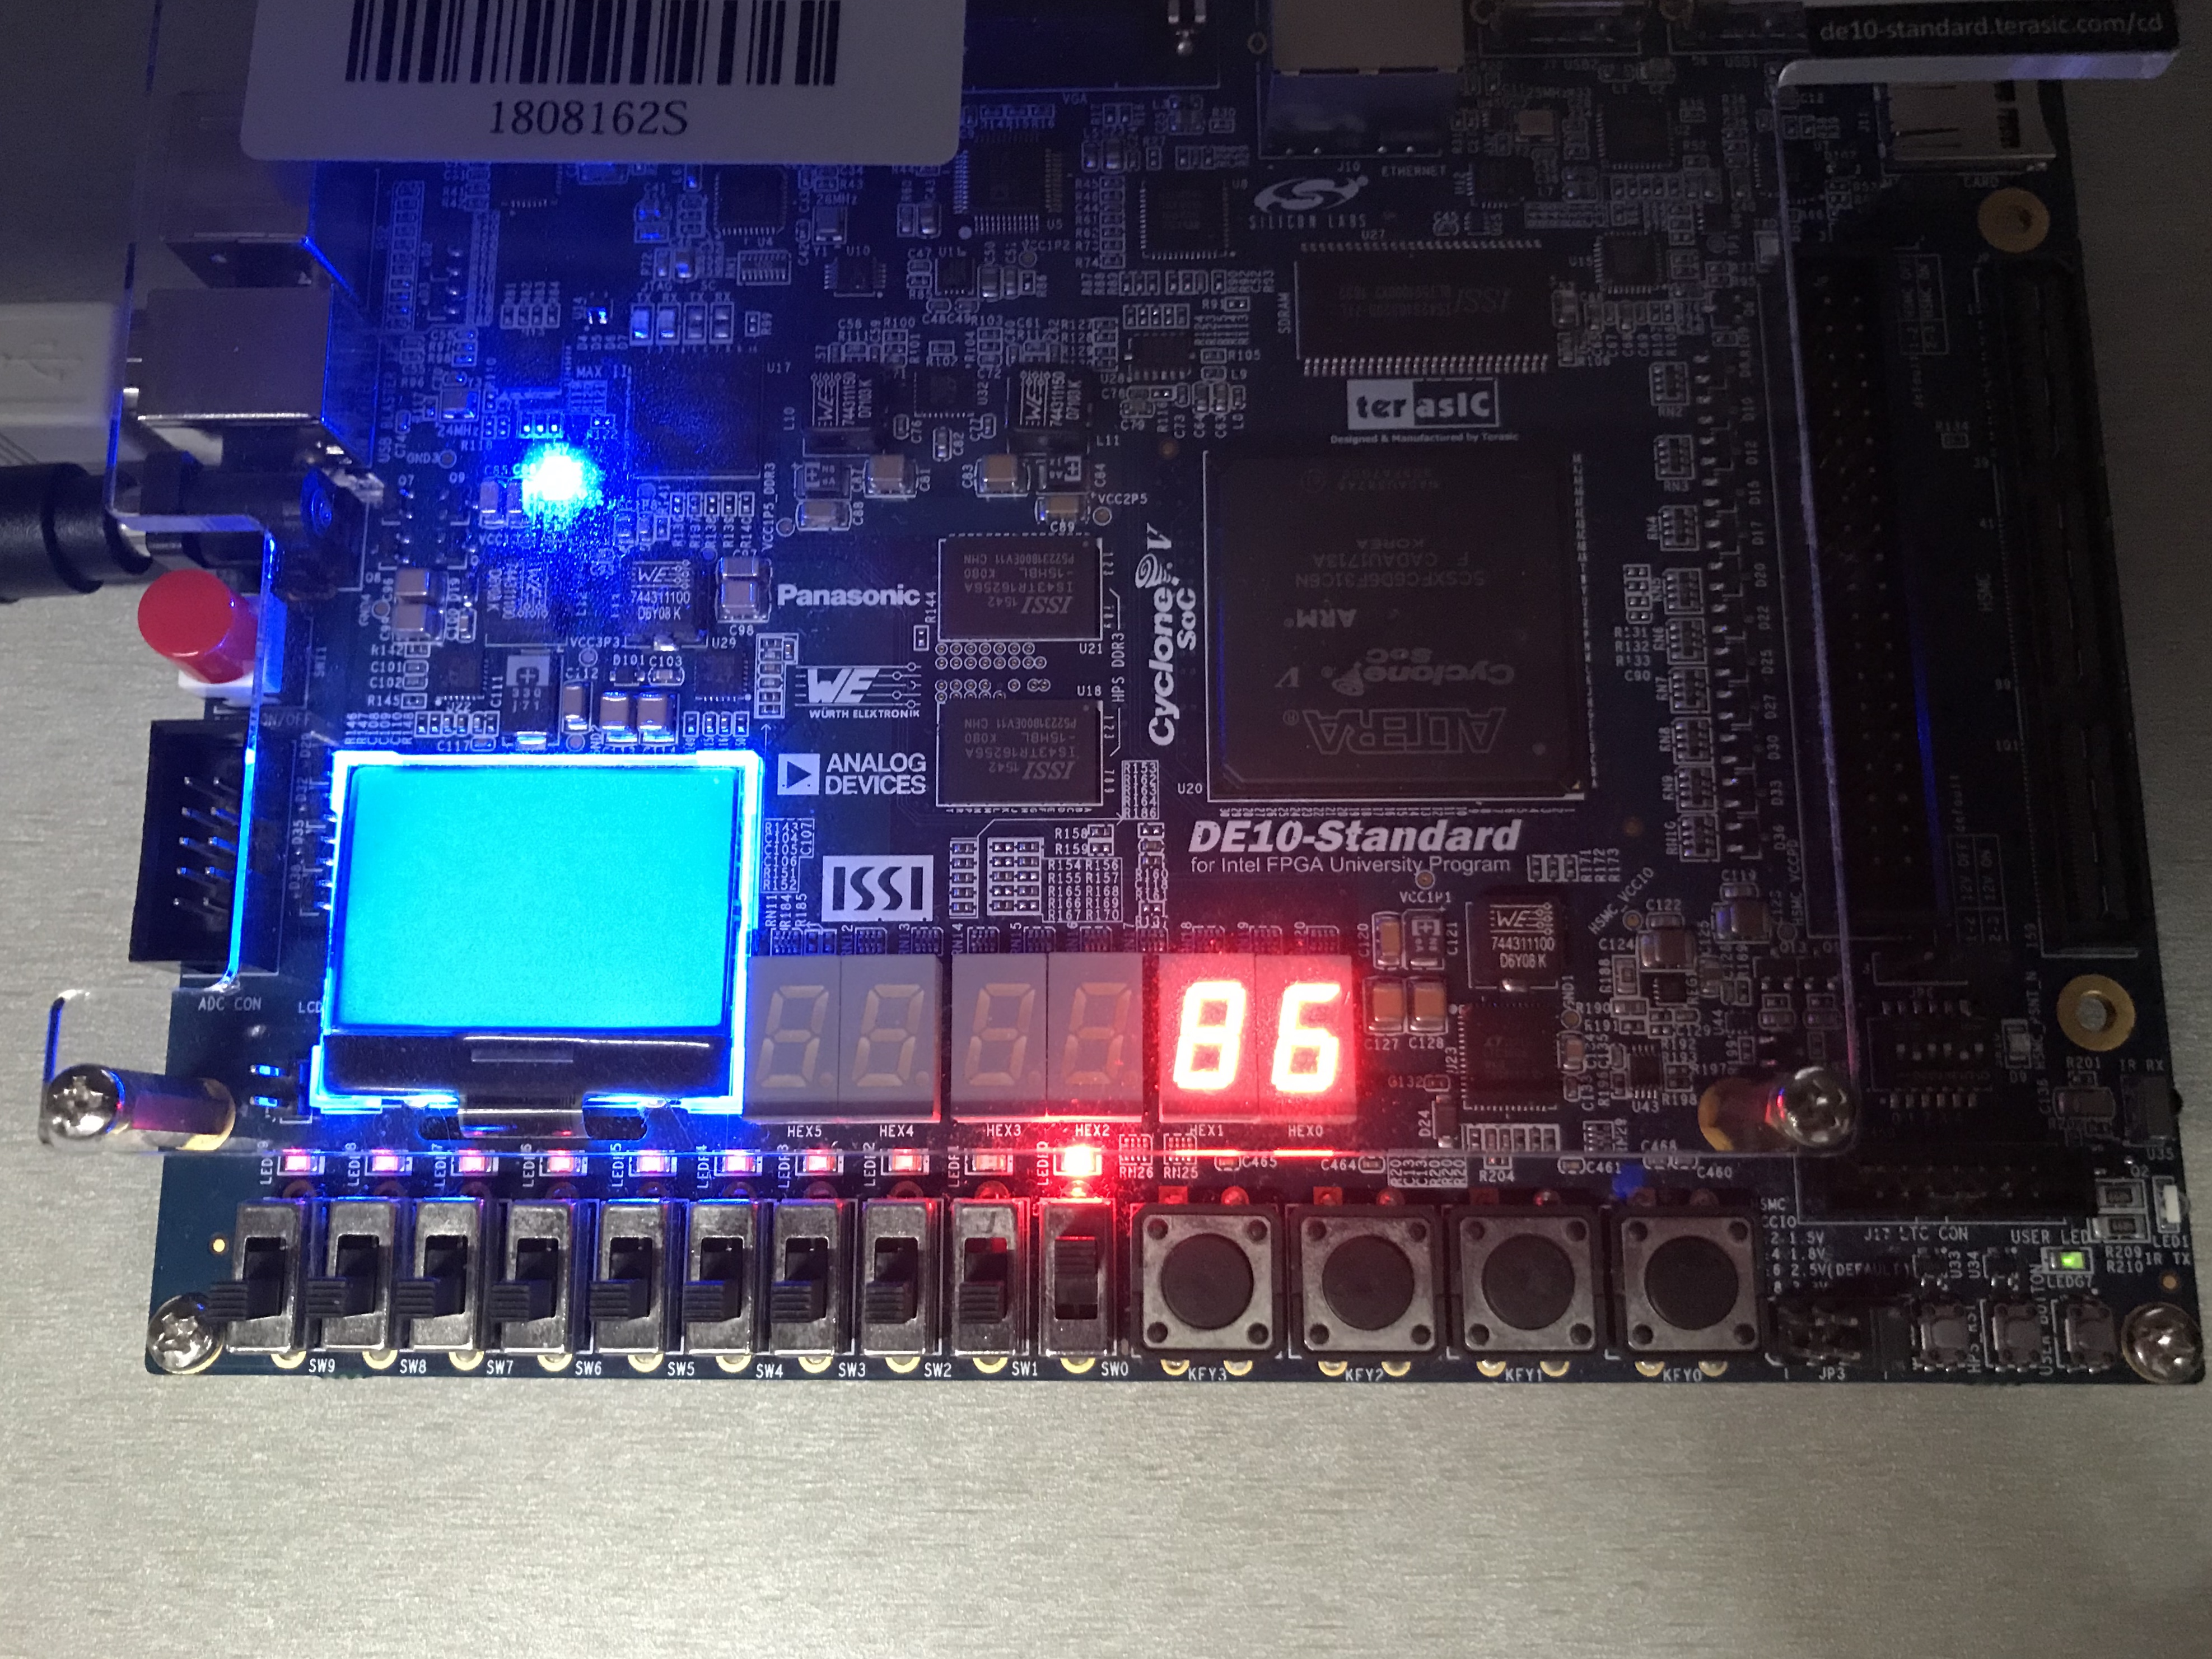
\includegraphics[width=1\textwidth]{1_fpga.jpg}
  \caption{实验5.4.1 下载运行(发光二极管亮表示暂停成功)}
  \label{1_fpga}
\end{figure}
\begin{figure}[H]
  \centering
  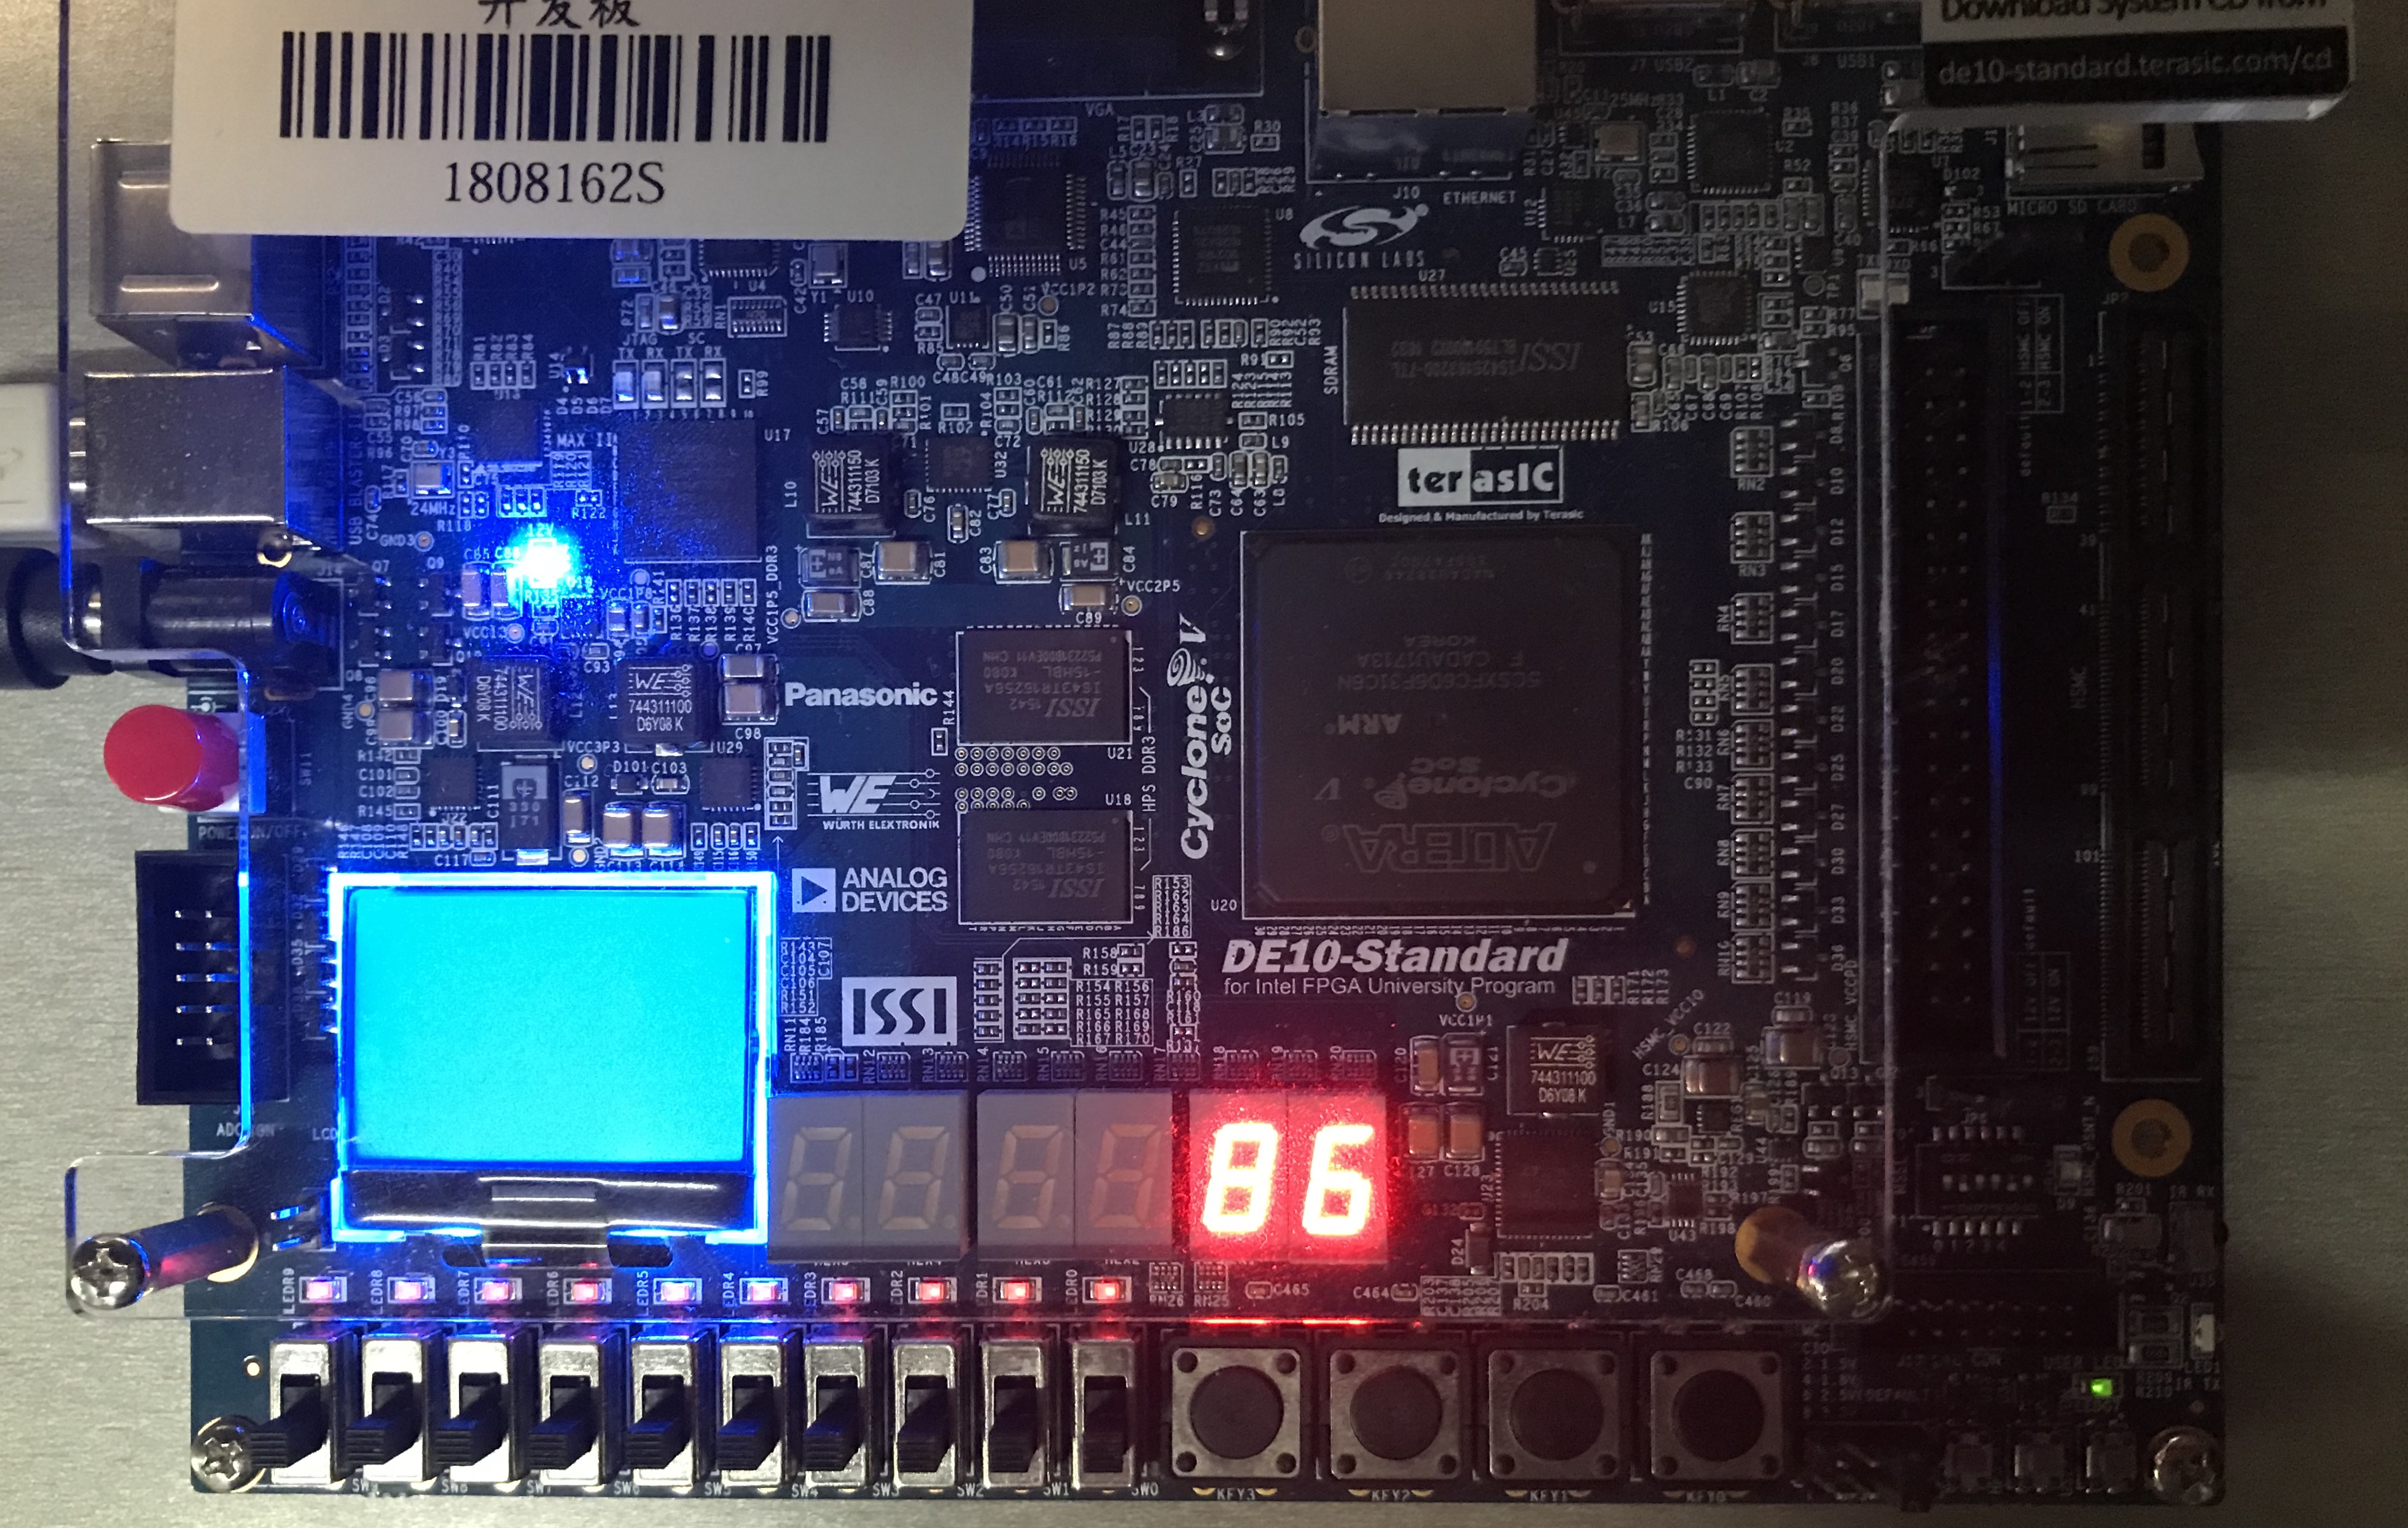
\includegraphics[width=1\textwidth]{2_fpga.JPG}
  \caption{实验5.4.2 下载运行(发光二极管亮表示闹钟已触发)}
  \label{2_fpga}
\end{figure}


\section{遇到的问题及解决办法}
\begin{itemize}
  \item 给七段数码管赋值应该在clk\_1s的
        上升沿赋值,要用非阻塞赋值语句
  \item 以25000000个脉冲周期为一秒进行仿真运行非常困难
        (具体怎样个困难法,详见实验5.4.1的测试文件部分。
        把``if (count\_clk == 25000000)''\linebreak[4]
        改成``if (count\_clk == 10)''再进行仿真会舒服很多
        (要记得在下载运行之前改回来啊啊啊)
  \item 同一信号不能在多个always块中赋值(低级错误++)
  \item 在测试文件中,如果仿真运行所要观测的时间较长的话,
        时钟信号的精确度会下降。例如当timescale是1 ns/1 ps、
        测试文件中自定义的CLOCK周期为1个时钟周期(1 ns)、
        而仿真运行时间为几千纳秒时,自定义的CLOCK就不那么精确了,
        可以根据测试需要手动调整\linebreak[4]
        initial中的等待时间``\#时间;''
\end{itemize}

\section{得到的启示}
\begin{itemize}
  \item 计数器原来可以用触发器实现
  \item 只有遇到问题才会得到启示,所以本条目可以归并到
        条目``遇到的问题及解决办法''中。
        \sout{(奇怪的启示增加了)}
  \item 上面的那句话是个悖论
\end{itemize}

\section{意见和建议}
\begin{itemize}
  \item 表5-1的表头有误(``减法计数器''写成了``加法计数器'')
  \item 从这个实验开始,就没有贴心又详细的手把手Verilog
        教程了吗(哭)?只给出实验题目描述,然后自己造代码
        的时代就要来临了吗?T\_T
\end{itemize}

\end{document}